\documentclass[ms,twoside,print]{nuthesis}
% Note: Leaving out print or twoside will result in oneside printing.

% Include necessary packages
\usepackage{amsmath}
\usepackage{amsfonts}
\usepackage[sc,osf]{mathpazo}
\usepackage{microtype}
\usepackage{booktabs}
\usepackage{paralist}
\usepackage{graphicx}
\usepackage{color}
\definecolor{dark-red}{rgb}{0.6,0,0}
\definecolor{dark-green}{rgb}{0,0.6,0}
\definecolor{dark-blue}{rgb}{0,0,0.6}
\interfootnotelinepenalty=10000 % This helps to prevent breaking footnotes across pages

% Load memhfixc after hyperref to fix issues with hyperref in memoir
\usepackage[
    pdfauthor={Andrei Modiga},
    pdftitle={Developing an AI-Assisted Grading System Using Large Language Models},
    pdfsubject={Education and AI},
    pdfkeywords={LaTeX, Project Proposal, AI, Education, Grading},
    linkcolor=dark-blue,
    pagecolor=dark-green,
    citecolor=dark-blue,
    urlcolor=dark-red,
    colorlinks=true,
    backref,
    plainpages=false, % This helps to fix the issue with hyperref with page numbering
    pdfpagelabels % This helps to fix the issue with hyperref with page numbering
]{hyperref}
\usepackage{memhfixc}

\begin{document}

% Start formatting the first few special pages
\frontmatter

% Title and author information
\title{Developing an AI-Assisted Grading System Using Large Language Models (GPT-4)}
\author{Andrei Modiga}
\adviser{Scot Anderson, Ph.D.}
\adviserAbstract{Scot Anderson, Ph.D.}
\major{Computer Science}
\degreemonth{August}
\degreeyear{2024}

% Optional fields (uncomment and modify if needed)
% \college{School of Computing}
% \city{Collegedale, Tennessee}

\doctype{PROJECT PROPOSAL}

\maketitle

\begin{abstract}
Grading written student work is a critical component of education, directly influencing the learning experience and providing essential feedback to both students and educators. This project focuses on building an AI-assisted grading system that leverages Large Language Models (LLMs), specifically GPT-4, to automate and enhance the grading process. By classifying student responses based on semantic similarity, the system streamlines grading and allows educators to provide more consistent and efficient feedback. The project aims to reduce the manual workload on teachers, improve grading consistency, and provide timely feedback to students.
\end{abstract}

%% The Table of Contents is required
\setcounter{tocdepth}{2} % Adjust this number to control the depth of the Table of Contents
\tableofcontents
\listoffigures
\listoftables

%% Main content starts here
\mainmatter

\chapter{Introduction}
In the educational landscape, grading written student work is a task of high importance; it directly influences the learning experience and provides crucial feedback to both students and educators. Traditional grading methods, while effective, can be time-consuming and labor-intensive, especially for teachers managing large volumes of student submissions. The demand for efficient and scalable grading solutions has become increasingly evident as educators seek to streamline their workloads without compromising assessment quality.

Recent advancements in artificial intelligence, particularly in the development of Large Language Models (LLMs), offer a promising approach to this challenge. LLMs like OpenAI's GPT-4 have demonstrated remarkable proficiency in processing and generating human-like text by analyzing vast datasets and recognizing patterns in language. These models have the potential to transform the grading process by automating the evaluation of student responses, thereby reducing the workload on teachers.

This project explores the development of an AI-assisted grading system that incorporates GPT-4 to classify student responses by grouping those that are semantically similar. By identifying clusters of answers that convey the same meaning, regardless of phrasing or structure, the system can assist educators in grading more efficiently.

The primary goal of this project is to build and implement this AI-assisted grading system, including the ability to recognize handwritten text, and integrate it into the educational platform, OICLearning.com. By focusing on building a practical solution, the project aims to enhance the grading process, making it quicker and more consistent, thereby allowing teachers to focus on more critical aspects of instruction while ensuring that students receive fair and accurate feedback.

However, integrating LLMs into the grading process presents challenges that must be carefully addressed. Key considerations include the model's ability to accurately differentiate nuanced meanings and appropriately group responses that, while semantically similar, may vary in correctness. Additionally, the effectiveness of these models in handling a diverse range of student expressions and potential errors needs thorough evaluation.

\chapter{Background}

The integration of artificial intelligence (AI) into education has revolutionized teaching and learning processes. A significant area of impact is the automation of grading, where AI technologies, particularly Large Language Models (LLMs) like GPT-4, have shown great promise. This chapter delves into the advancements in AI-assisted grading, focusing on GPT-4's role, and discusses existing research, challenges, and the potential benefits of such systems.

\section{Artificial Intelligence in Education}

Artificial intelligence has become a significant part of modern education, offering tools and solutions that enhance learning experiences and streamline administrative tasks. AI-driven educational platforms can personalize learning paths, adapt content to individual student needs, and provide real-time feedback~\cite{Alto2023}. This personalization is crucial in accommodating diverse learning styles and improving student engagement.

Moreover, AI systems can analyze vast amounts of data to identify patterns and trends in student performance. Teachers can use these insights to tailor instruction, address knowledge gaps, and improve overall educational outcomes. The automation of administrative tasks, such as scheduling and attendance tracking, allows teachers to focus more on instruction and less on paperwork~\cite{Chen2020}.

\subsection{Personalized Learning and Feedback}

One of the most significant contributions of AI in education is the ability to offer personalized learning experiences. Intelligent tutoring systems powered by AI can adjust the difficulty level of exercises based on a student's performance, ensuring optimal learning progression~\cite{Alto2023}. These systems can also identify areas where a student is struggling and provide targeted interventions.

In the context of grading, AI can provide detailed feedback on assignments, highlighting specific areas of strength and weakness. GPT-4, for instance, can generate personalized comments that help students understand their mistakes and learn from them. This immediate and individualized feedback is more effective than generic responses and can significantly enhance the learning process~\cite{Luckin2016}.

\subsection{Administrative Efficiency}

AI's ability to automate routine administrative tasks is transforming the educational landscape. Tasks such as grading, scheduling, and record-keeping can be handled efficiently by AI systems, reducing the workload on educators~\cite{Alto2023}. This automation not only saves time but also minimizes human errors that can occur in manual processes.

Furthermore, AI systems can monitor student engagement and participation, alerting educators to potential issues such as decreased performance or absenteeism. By identifying these problems early, interventions can be implemented promptly, supporting student retention and success~\cite{Zawacki2021}.

\section{Advancements in Large Language Models}

\subsection{Introduction to GPT-4}

GPT-4, developed by OpenAI, is one of the most advanced LLMs available today. Building upon the success of its predecessors, GPT-4 has been trained on an extensive dataset comprising diverse textual content, enabling it to understand and generate human-like text with remarkable fluency and coherence~\cite{Alto2023}.

The architecture of GPT-4 allows it to capture complex language patterns, understand context, and infer meaning beyond surface-level interpretations. This deep understanding is particularly beneficial in educational applications where more than simple comprehension of student responses is required.

\subsection{GPT-4 in Educational Applications}

GPT-4's capabilities extend to various educational applications. It can assist in content creation, such as generating lesson plans, educational materials, and practice questions tailored to specific learning objectives~\cite{Alto2023}. In language learning, GPT-4 can provide conversational practice, corrections, and explanations to learners.

In grading, GPT-4's ability to understand and evaluate open-ended responses makes it a valuable tool. It can analyze essays, short answers, and problem-solving explanations, providing not only grades but also constructive feedback. This level of assessment requires a deep understanding of the subject matter and the ability to interpret diverse student expressions~\cite{Lund2023}.

\section{AI-Assisted Grading Using GPT-4}

\subsection{Automating Short Answer Grading}

Short answer questions are challenging to grade automatically due to the variability in student responses. Traditional grading systems rely on keyword matching or predefined answer patterns, which can miss correct answers phrased differently or accept incorrect answers that contain the right keywords.

GPT-4 overcomes these limitations by understanding the semantic meaning behind the text. It can recognize correct answers even when they are expressed in unconventional ways and identify incorrect answers that superficially appear correct~\cite{Liu2023}. This semantic understanding allows for more accurate grading of open-ended questions.

Liu et al.~\cite{Liu2023} conducted a study demonstrating GPT-4's effectiveness in grading university-level mathematics exams. The AI model was able to evaluate complex mathematical reasoning and provide grades that closely aligned with human graders. This study highlights GPT-4's potential in handling subjects that require critical thinking and problem-solving skills.

\subsection{Grading Handwritten Responses}

Grading handwritten assignments poses additional challenges due to the need for accurate handwriting recognition. Optical Character Recognition (OCR) technologies have improved, but they still struggle with illegible handwriting or complex symbols commonly used in subjects like mathematics and physics.

Kortemeyer (2023)~\cite{Kortemeyer2023} explored the feasibility of using AI to grade handwritten physics solutions. By integrating OCR technologies with GPT-4, the study achieved a significant correlation between AI-generated grades and human grading. However, the study also noted limitations in accurately interpreting diagrams and notations, indicating areas where further improvement is needed.

\subsection{Semantic Understanding and Contextual Evaluation}

GPT-4's advanced natural language processing capabilities enable it to understand context and semantics deeply. It can evaluate not just the correctness of an answer but also the reasoning process behind it. This is important in subjects where the method is as important as the final answer, such as mathematics and science.

For example, GPT-4 can assess a student's problem-solving approach, identify logical errors, and provide specific feedback on where the reasoning went astray~\cite{Alto2023}. This level of detailed evaluation helps students understand their mistakes and learn more effectively.

\section{Challenges in AI-Assisted Grading with GPT-4}

\subsection{Accuracy and Reliability}

While GPT-4 demonstrates high proficiency in understanding and evaluating text, it is not immune to errors. Misinterpretations can occur, especially with ambiguous or poorly constructed responses. Liu et al. (2023)~\cite{Liu2023} emphasized the importance of human oversight to ensure the reliability of AI-generated grades.

Moreover, AI models may sometimes be overconfident in their assessments, potentially leading to incorrect grading. Implementing mechanisms for uncertainty estimation and flagging ambiguous cases for human review can mitigate this issue.

\subsection{Bias and Fairness}

AI models can inadvertently exhibit biases present in their training data. This raises concerns about fairness, as certain groups of students might be disadvantaged by biased grading. Tossell et al. (2023)~\cite{Tossell2023} highlighted the importance of addressing these biases to ensure equitable treatment of all students.

Strategies to mitigate bias include using diverse and representative training data, implementing fairness-aware algorithms, and regularly auditing AI systems for discriminatory patterns~\cite{Mehrabi2021}.

\subsection{Handwriting Recognition Limitations}

Despite advancements in OCR technologies, accurately recognizing handwritten text remains challenging. Variations in handwriting styles, the use of non-standard symbols, and poor scan quality can hinder recognition accuracy.

Kortemeyer et al. (2023)~\cite{Kortemeyer2023b} found that AI struggled with interpreting hand-drawn diagrams and complex notations, which are common in STEM subjects. Improving OCR algorithms and combining them with context-aware models like GPT-4 can enhance performance, but human intervention may still be necessary in some cases.

\subsection{Ethical and Privacy Concerns}

The use of AI in grading involves processing sensitive student data, raising ethical and privacy considerations. Compliance with regulations such as the Family Educational Rights and Privacy Act (FERPA)~\cite{ferpa} is essential.

Alto (2023)~\cite{Alto2023} emphasizes the need for robust data protection measures, transparency in AI operations, and obtaining informed consent from users. Ensuring that AI systems are secure and that data is handled responsibly is crucial for maintaining trust.

\section{Existing Research on AI Grading Systems}

\subsection{Machine Learning Approaches}

Before the advent of LLMs like GPT-4, machine learning approaches to grading primarily involved training models on labeled datasets to recognize correct answers. Weegar and Idestam-Almquist (2022)~\cite{Weegar2022} explored such methods for grading short answers in computer science exams.

Their research demonstrated that machine learning could significantly reduce grading workload by clustering similar answers and automating scoring. However, these systems often required extensive preprocessing and were limited in handling the full variability of human language.

\subsection{Feasibility Studies with GPT-4}

Studies utilizing GPT-4 have shown promising results in various subjects. Kortemeyer (2023)~\cite{Kortemeyer2023} conducted a feasibility study on using GPT-4 for grading physics problems. The AI's grades correlated highly with human graders, indicating its potential effectiveness.

However, the study also noted that GPT-4 sometimes missed nuanced aspects of the solutions, particularly in assessing the quality of reasoning and the appropriateness of assumptions. This suggests that while GPT-4 can assist in grading, it should complement rather than replace human judgment.

\subsection{Student Perceptions of AI Grading}

The acceptance of AI-assisted grading by students is crucial for its successful implementation. Tossell et al. (2023)~\cite{Tossell2023} examined student perceptions of using AI tools like ChatGPT in academic settings.

While students appreciated the promptness and consistency of AI feedback, they expressed concerns about the transparency of the grading process and the AI's ability to understand their unique perspectives. Building trust requires clear communication about how the AI operates and opportunities for students to contest or discuss their grades~\cite{Zawacki2021}.

\section{Potential Benefits of GPT-4 in Grading}

\subsection{Efficiency and Scalability}

Implementing GPT-4 in grading systems can significantly reduce the time educators spend on evaluating assignments. This is especially beneficial in large classes where manual grading is impractical. AI systems can handle vast amounts of data quickly, providing timely feedback to students~\cite{Alto2023}.

\subsection{Consistency and Fairness}

AI grading systems apply the same criteria uniformly, reducing inconsistencies that can arise from human graders' subjective judgments or fatigue. This consistency contributes to fairness, ensuring that all students are evaluated on the same basis~\cite{Konnecke2020}.

\subsection{Timely Feedback}

Prompt feedback is essential for effective learning. AI systems can provide immediate evaluations, allowing students to understand their performance and address any issues while the material is still fresh in their minds~\cite{Nicol2006}.

\subsection{Enhanced Learning Outcomes}

By analyzing patterns in student responses, AI systems can identify common misconceptions and areas where many students struggle. Educators can use this information to adjust their teaching strategies, focus on problematic topics, and improve overall learning outcomes~\cite{Zawacki2021}.

\section{Summary}

The integration of GPT-4 into grading systems offers significant advantages, including increased efficiency, consistency, and the ability to provide personalized feedback. While challenges such as accuracy, bias, and ethical considerations exist, ongoing research and development are addressing these issues.

By combining GPT-4's capabilities with human oversight and ethical practices, AI-assisted grading can enhance educational experiences for both students and educators. The potential for improved learning outcomes and reduced workloads makes this an important area of development.

\section{Conclusion}

The existing body of research highlights the transformative potential of AI-assisted grading using GPT-4. By understanding the capabilities and limitations of these systems, educators can implement AI tools that complement their teaching practices.

The proposed AI-assisted grading system aims to build upon this foundation, addressing current challenges and harnessing GPT-4's full potential. By doing so, it seeks to improve the grading process, enhance learning experiences, and contribute to the advancement of AI in education.

\chapter{Proposal}

This chapter outlines the key requirements for developing an AI-assisted grading system using Large Language Models (LLMs) like GPT-4 and GPT-4 Vision, implemented in Python. The goal is to automate the grading process for various types of assignments on OICLearning.com by utilizing GPT-4 Vision to read images directly, performing both Optical Character Recognition (OCR) and Natural Language Processing (NLP) in a unified model. Additionally, the system will incorporate grading algorithms to assign grades based on expected answers for each question. This integration simplifies the workflow and enhances the system's ability to accurately interpret and grade student submissions.

\section{Summary of Requirements}

The AI-assisted grading system will require the development of both backend and frontend components. The backend will handle the processing of student submissions, including images and text, and communicate with GPT-4 and GPT-4 Vision via API calls. The frontend will provide an interface for instructors to review, sort, and manage graded assignments.

Key requirements include:

\begin{itemize}
    \item \textbf{Backend API Development:} Implement a backend API in Python that can receive images and text submissions from students and send them to GPT-4 and GPT-4 Vision for 
    processing.
    %% Summary - this is covered in the previous point. 
    %\item \textbf{Integration with GPT-4 Vision:} Utilize GPT-4 Vision's capabilities to perform OCR and NLP on images of student submissions.
    % \item \textbf{Grading Algorithm:} Develop algorithms to compare the processed student responses against expected answers and assign appropriate grades.
    \item \textbf{Frontend Interface:} Create a user-friendly frontend interface that allows instructors to view, sort, and manage the process of grading assignments.
    \item \textbf{Data Security and Privacy:} Ensure the system complies with data protection regulations, implementing necessary security measures.
    \item \textbf{Scalability:} Design the system to handle a large number of student submissions and various types of assignments.
    \item \textbf{User Authentication:} Integrate with the secure login and access control mechanisms avaialable in the OICLearning.com project.
\end{itemize}

\section{Proposed Approach}

The proposed AI-assisted grading system will be implemented using a modular architecture, separating the backend processing from the frontend user interface. The backend will be developed in Python and will utilize the OpenAI API to interact with GPT-4 and GPT-4 Vision. The system will process images submitted by students, perform OCR to extract text, and then use NLP to interpret the content.

\subsection{Backend Implementation}

The backend API will handle the following tasks:

\begin{itemize}
    \item Receive images and text submissions from the frontend.
    \item Send images to GPT-4 Vision via API calls for OCR and NLP processing.
    \item Parse and handle responses from GPT-4.
    \item Compare the interpreted responses to predefined expected answers. %Dr. A says, OK this may be needed to do accurate grouping.
    \item Store the results in a database.
\end{itemize}

\subsection{Frontend Development}

The frontend will be a web-based application that allows users to:

\begin{itemize}
    \item Securely log in to the system.
    \item Upload and submit assignments. %Added by Dr. A
    \item View graded assignments and student responses.
    \item Sort and filter submissions based on various criteria (e.g., grade, date submitted).
    \item Calculate grades based on a grading rubric or algorithm.
    \item Override grades or make manual adjustments.
\end{itemize}

\subsection{System Integration}

By leveraging GPT-4 Vision's capabilities, the system simplifies the grading workflow by handling both OCR and NLP tasks within a single model, reducing complexity and potential points of failure. The modular design allows for scalability and ease of maintenance.

\section{Detailed Requirements and User Stories}

Four user stories describe the processes that drive the requirements. These stories include: the teacher creating an assignment, teachers or students uploading submissions, the AI assisted grading of assignments and finally the teacher transfering the grades to an Learning Management system (LMS). These stories and their associated requirements describe a series of webpages shown in Figure~\ref{fig:page-flow}  The following sections detail each of these stories.

\begin{figure}[h]
    \centering
    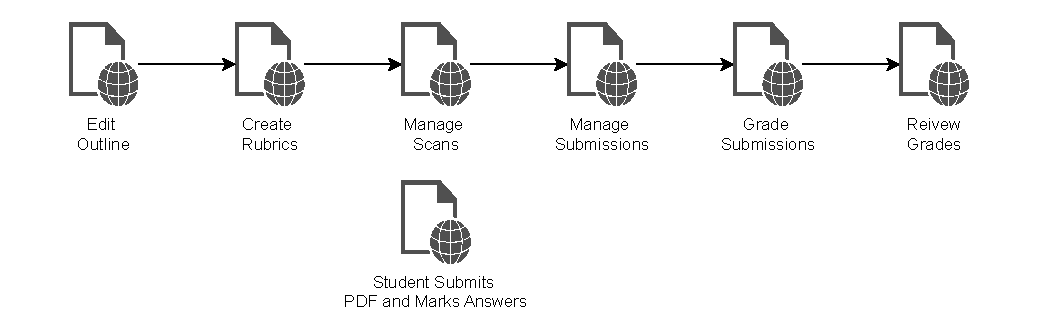
\includegraphics[width=.95\textwidth]{images/page-flow.pdf}
    \caption{Page flow diagram showing the sequence of pages in the system.}
    \label{fig:page-flow}
\end{figure}

\subsection{A teacher creates an assignment}

When a teacher creates an assignment, they choose from different kinds of AI assisted types. These types include:

\begin{itemize}
    \item Filled-Form that students write on and are later scanned in by the teacher. E.g. a written test. 
    \item Free-Form typed or written assignments where the location of answers may vary. E.g. an assignment that is given to the students in a word document and the length of their answer may vary, and hence their location may vary.
    \item Online Filled-form assignments. E.g. a quiz that is taken online where answers that contains digital responses from students. This is not within the scope of this project.
\end{itemize}

For Filled-Form type assignments, the teacher needs to prompt the system by uploading a blank of the form. Figure~\ref{fig:filled-form} shows an example of what this page might look like. The teacher first identifies the location of the student identity (name and/or ID number). In the Figure, this is shown by the tan box added by the teacher around the area where a student is instructed to place their name. To add a question, the teacher clicks on the ``New Question'' link at the bottom right. The system adds a new question to the list and an associated box to go with it. Then the teacher must: name the question, assign points, locate and size the associated box (shown in green) of the answer area over the blank spot they expect students to write in, and give the expected answer (not shown). Figure~\ref{fig:filled-form} shows the name area and a single question where the teacher can accomplish all these things. Here when a teacher clicks on a question in the list, they can edit the box size/location along with the name or points. The plus sign next to the red X, allows the teacher to add a sub-question. Sub-questions work the same way as questions except they appear as a sublist under the question.

\begin{figure}[htb]
    \centering
    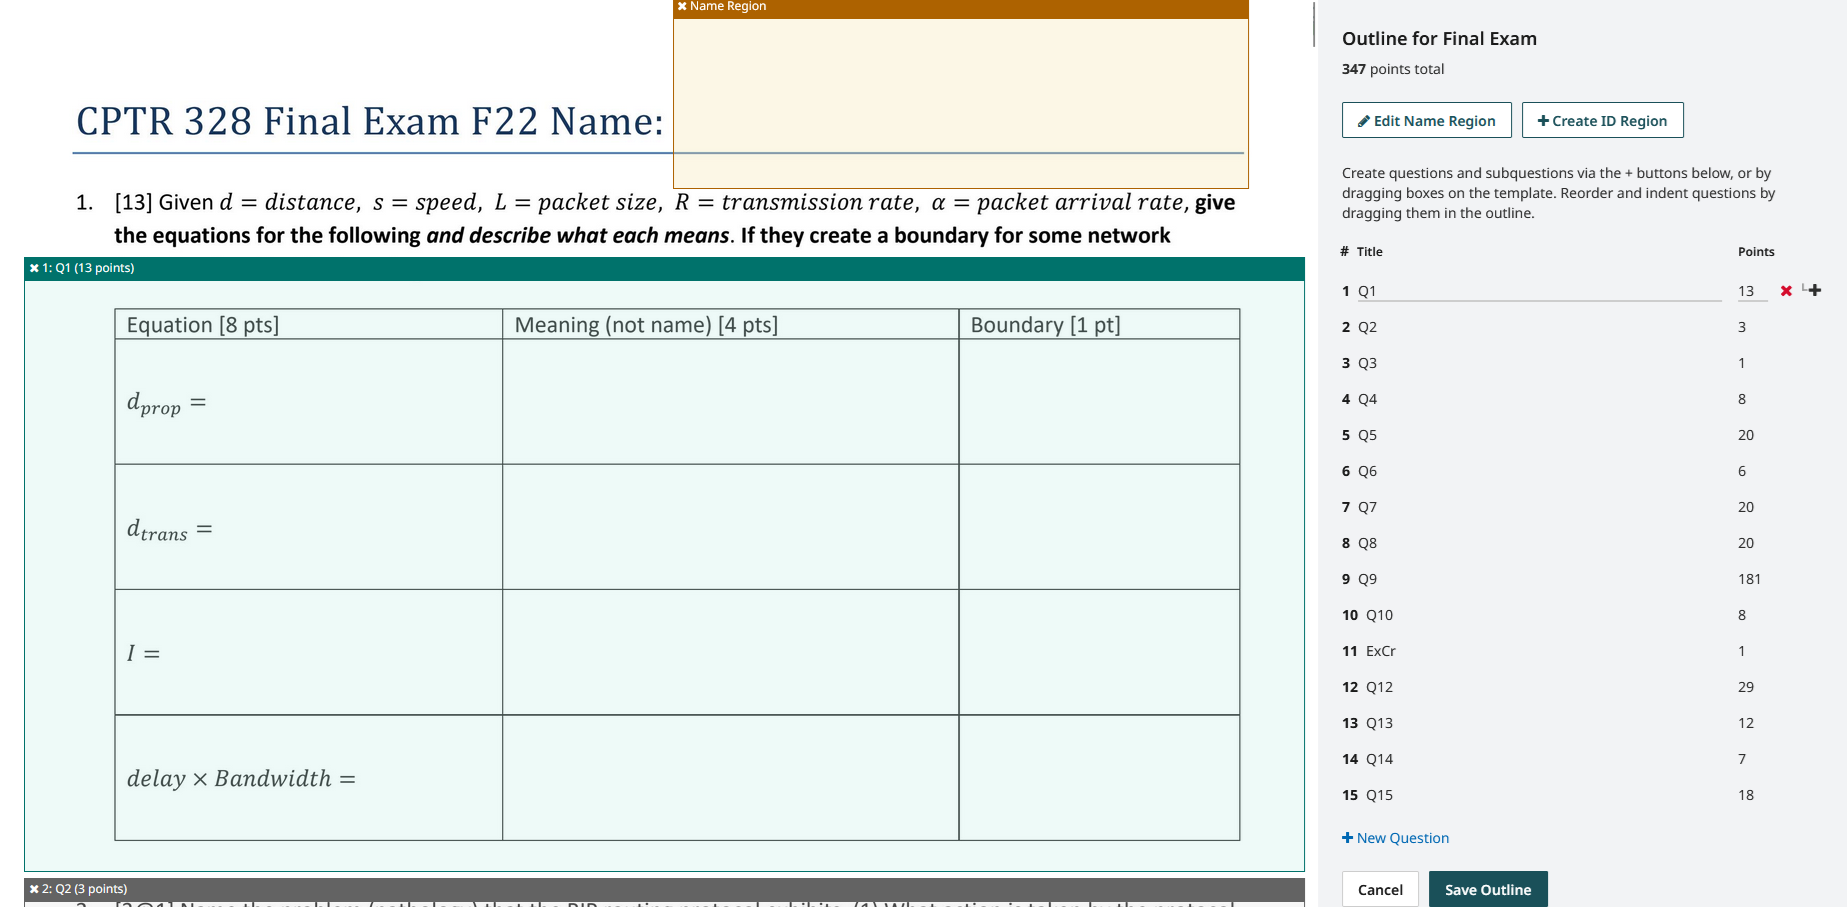
\includegraphics[width=\textwidth]{images/filled-form-creation.png}
    \caption{The filled-form assignment creation page.}
    \label{fig:filled-form}
\end{figure}

This process is called ``editing the outline'' and includes everything the system needs to define the assignment. The teacher can then save the outline and the system will be ready to accept student submissions. The teacher can create rubrics at this point or, more likely, defer this step until grading. If the teacher decides to create the rubrics now, they progress to the webpage called ``Create Rubrics'' (see Figure~\ref{fig:page-flow}). Otherwise, they can add rubrics during grading.

A rubric scoring guide defines text describing the error with a value subtracted from a score when applied. The teacher can add up to 36 rubrics and they shall be numbered 0-9, and a-z. Teachers assign one or more rubrics to an answer (or group of answers when grading groups) during grading.  

In the case of Free-form typed or written assignments, the teacher gives the students questions, and the students turn in their answers as a PDF. Students may or may not include the questions, so the answer's location will vary from student to student. Here the teacher does not need to identify the location of an answer, but they do need to provide question identifiers and points for students to use when turning in the document. Figure~\ref{fig:free-form} shows an example of the teacher creating a Free-Form assignment. Notice that there is no need to draw a rectangle around the answer area and except for that task the teacher's work is identical to the filled-form assignment above.

\begin{figure}[htb]
    \centering
    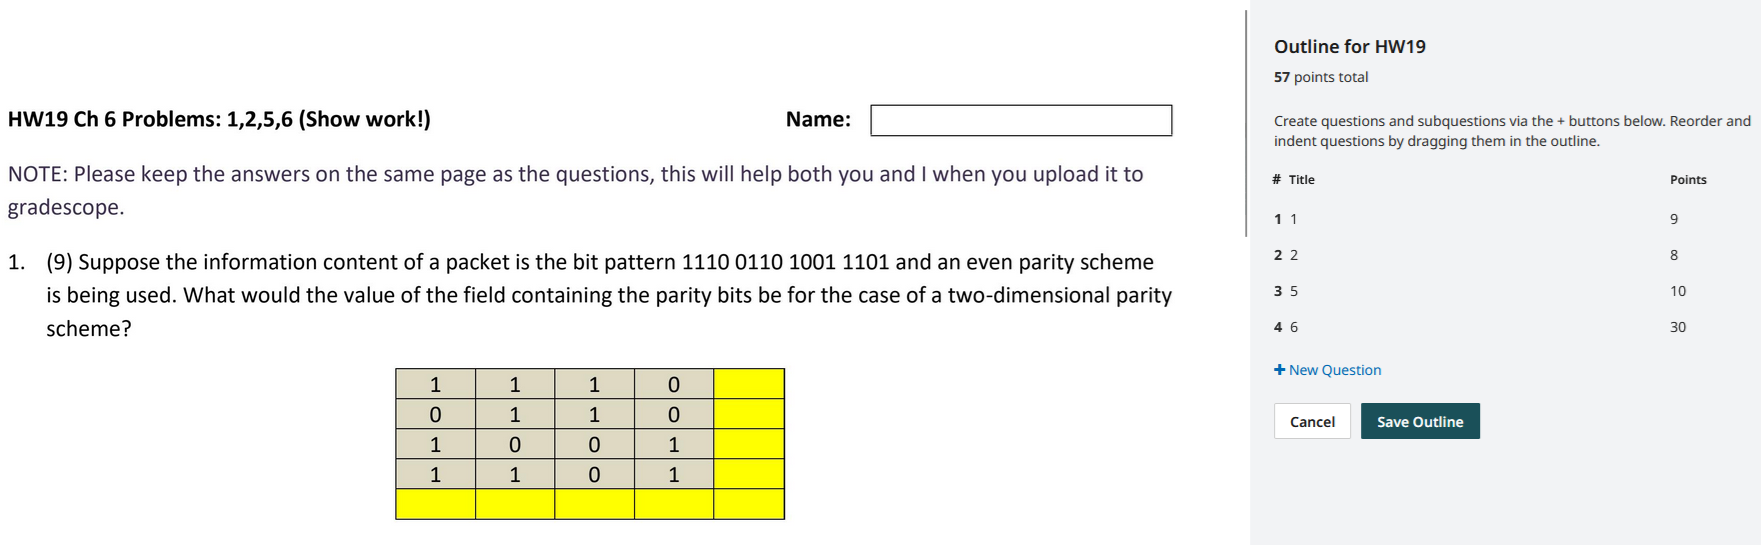
\includegraphics[width=\textwidth]{images/free-form-creation.png}
    \caption{The free-form assignment creation page.}
    \label{fig:free-form}
\end{figure}

\subsection{Preparing Submissions to be graded}

The two tasks at this stage are uploading submissions and assigning names to them. This is done in two steps. First, the assignments are uploaded by the teacher or by the individual student. Second, the teacher approves/assigns names to the assignments. This takes two screeens: Manage Scans and Manage Submissions, or one screen when uploaded by the student (refer to the pages list in Figure~\ref{fig:page-flow}).

\textit{Manage scans}: After a teacher has logged in and gone to a filled-in assignment, they upload all the assignments as a single PDF. The system already knows how many pages are in each assignment because it identified that number in the creation process above. The system separates the PDF into individual documents and attempts to assign the names of students based on the identity. This is accomplished on a screen called Manage. However, this page does not show the individual assignments or the names it has assigned. It only shows the number of assignments it assigned~\footnote{\scriptsize{In other grading systems, PDFs are converted to images. Although we would like to deal with PDFs natively, this is an acceptable solution}}. 

\text{Manage Submissions}: In this page, a teacher can view a portion of each submission that contains the identity of the student. The system knows the students in the class and populates drop-down selection boxes for the names of students that it could not identify. The teacher can then select the correct student name from the drop-down. Of course, this is only necessary for Filled-form assignments uploaded by the teacher. Free-form assignments that students upload are automatically assigned to the student that uploaded them. Consequently, Free-form assignments will not have this page in the list of pages teachers see to manage the assignment.  

\subsection{Grading Submissions}

The process starts with a list of questions for an assignment that needs grading. Each question is a link to a page where grouping can occur. The AI assists in this process by default, but the teacher can override the AI's grouping, or stop the process and manually group answers. 

In the AI assisted process, the screen shows the list of groups on the right with the main screen showing the student answers as images in a grid. Figure~\ref{fig:answer-grouping} shows an example with eight answers. The first three in the left column have been selected by clicking on the images, and at this point would form a new group if the user clicks on the ``+Create a Group'' button. The AI should group the results first, but may leave some in an uncategorized group. That is, single submissions that don't fit into a group need not be put in a separate group, but should be kept in an uncategorized group. \textit{All} groups should be listed at the right. When clicking on the group, the system should de-select any images currently selected and then show the newly selected group's images in the main page. When images are selected and the ``Create a Group'' button is clicked, the system should create the group and move the images from the current group to the new group, then display the new group and its images. 

\begin{figure}[htb]
    \centering
    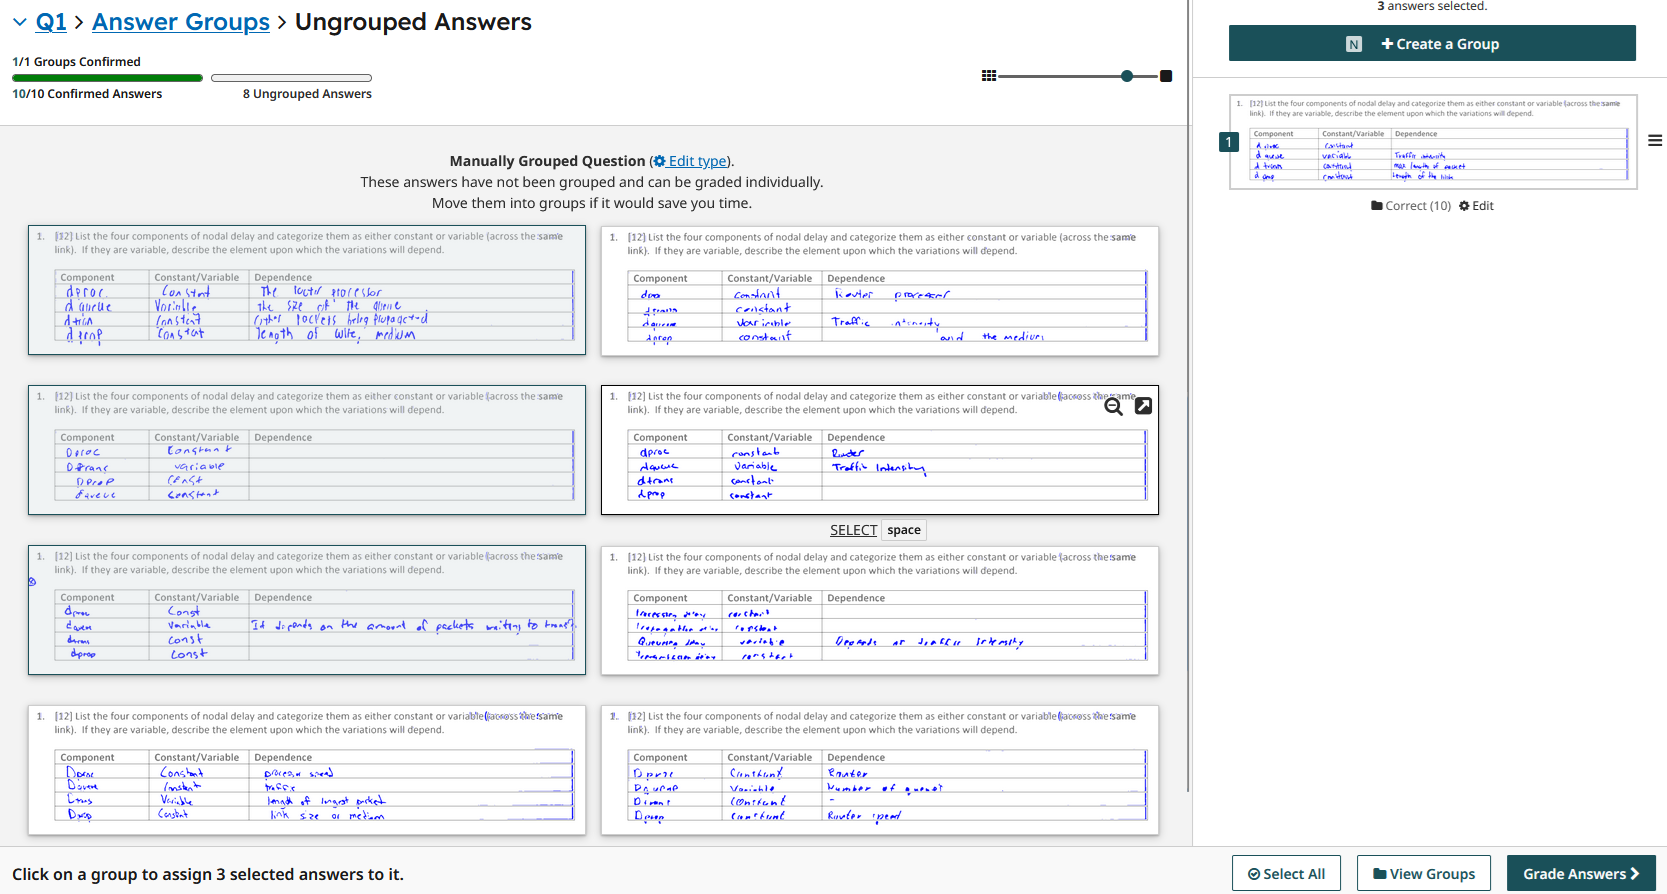
\includegraphics[width=0.95\textwidth]{images/grouping-answers.png}
    \caption{Grouping answers.}
    \label{fig:answer-grouping}
\end{figure}

Selecting a group shows the group's Information. This information includes the images in the group (in the main screen), the name of the group, the number of images in the group, and a description of the group. All of these are assigned by the AI and the teacher may edit these items as appropriate. 

Before moving to the next step it is important that the teacher review all the groups and that they are satisfied that the groups are correct. If the teacher decides that the grouping is incorrect, they must come back to this page to regroup them. 

Once the system has groups created, the teach can proceed to grade the answers. The teacher does this by clicking on the Grade Answers button at the lower right in Figure~\ref{fig:answer-grouping}. Groups are graded in order that they appear on the screen with the sole exception that no matter where the uncategorized group is, it is always graded last. 

When grading a group, the teacher is shown the group name, the number of images in the group, a sample answer(s) from the group, and the description of the group. The teacher can then assign rubrics that subtract points and provide feedback to students. The description of the group is part of the feedback that the student will see. Figure~\ref{fig:grading-answers} shows and example of what the grading page might look like. Several important requirements come into play for ease of use, specifically key presses and mouse movements have the following meaning:

\begin{figure}[htb]
    \centering
    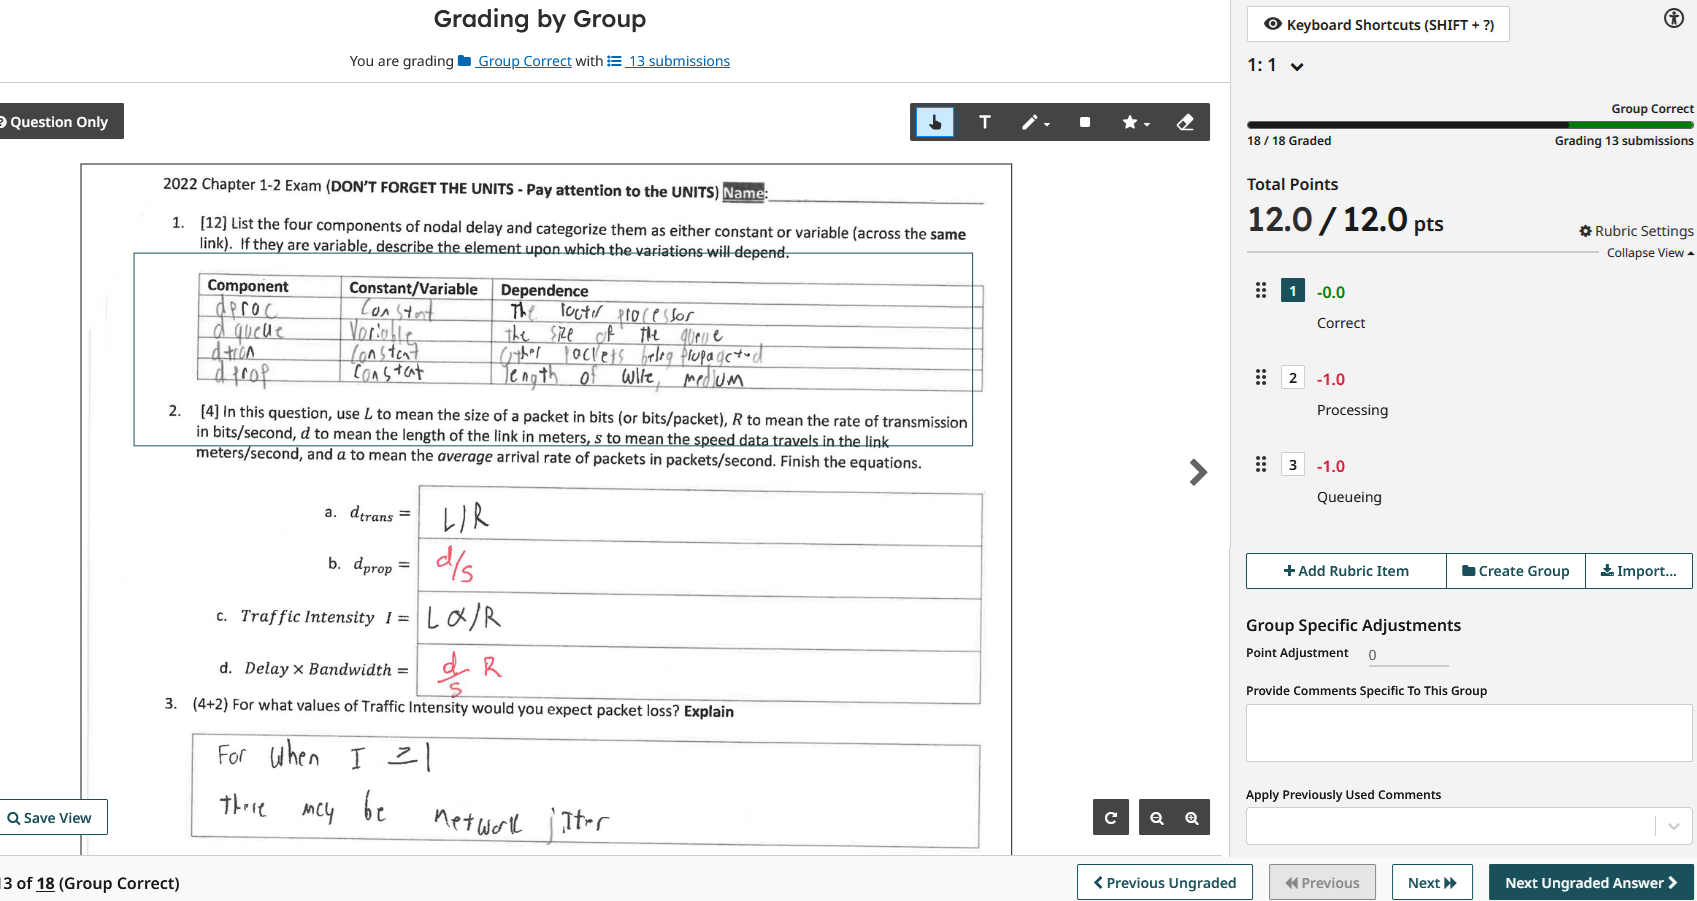
\includegraphics[width=0.95\textwidth]{images/grading-answer.png}
    \caption{The grading page.}\label{fig:grading-answers}
\end{figure}

\begin{itemize}
    \item Pressing 0--9 or some key combination with a--z toggles the rubric between assigned and not-assigned to the group. 
    \item Left arrow takes the teacher to the previous group or individual submission.
    \item Right arrow takes the teacher to the next group or individual submission.
    \item Scrolling up or down over the rubrics scrolls through the available rubrics.
    \item Scrolling on the image zooms in and out.
    \item Clicking and dragging the image moves it around in the viewing area. 
\end{itemize}

Suppose a teacher decides to change the value of a rubric. They can simple edit the rubric while grading and all grades where this rubric applies are updated with the new value.

When the teacher completes all of the groups and each individual assignment in the uncategorized group, they can move on to the next question in the assignment. When they are finished with all the questions, they can publish the results so that students can see them. This ``Review Grades'' page allows the teacher to see a list of all the grades has buttons to do the following actions:

\begin{itemize}
    \item Publish or Unpublish grades (Students see grades or not)
    \item Download Grades (export grades to an Excel or CSV file)
    \item Export submissions (to a zip file). Submissions are in PDF format and include the following:
    \begin{itemize}
        \item Name and Identifying information of the student along with the assignment score.
        \item A list of question names with the points assigned and the rubrics applied to that question. 
        \item After the grade information, The students original work is shown.
    \end{itemize}
    \item Export Evaluations (to a zip file of CSV files see Figure~\ref{fig:evaluation-export} for an example of a single question evaluation). 
\end{itemize}

\begin{figure}[htb]
    \centering
    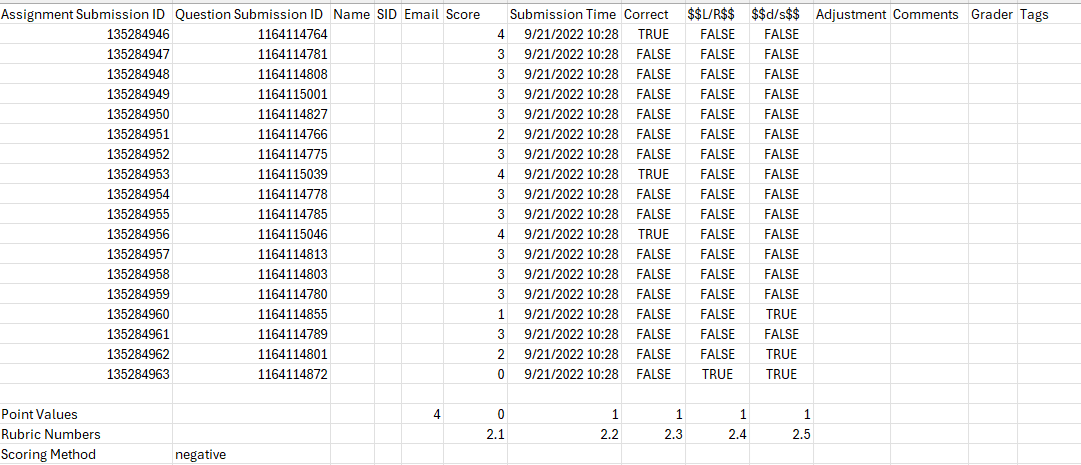
\includegraphics[width=\textwidth]{images/evaluation-exports.png}
    \caption{Comma separated values (CSV) file example.}\label{fig:evaluation-export}
\end{figure}

This naturally brings us to the last step, transferring grades to an LMS.

\subsection{Transferring Grades to an LMS}

For the time being, this means downloading an Excel or CSV file that includes the student identifying information and the grade (e.g. 11/15) and a percentage (e.g. 73) without the percent sign. The teacher can then upload this file to the LMS.

\section{Final Deliverables}

Upon completion of the project, the following deliverables will be provided:

\begin{itemize}
    \item Fully functional AI-assisted grading system integrated with OICLearning project.
    \item Source code for both backend and frontend components.
    \item Technical documentation detailing system architecture, setup, and usage.
    \item User guide for instructors on how to use the system.
    \item Test cases and testing reports.
    \item Deployment scripts and configuration files.
\end{itemize}

\chapter{Testing}

We plan to conduct targeted testing activities to ensure that the system meets its key objectives. The testing will focus on verifying \emph{functionality}, \emph{accuracy}, and \emph{usability}.

\section{Planned Testing Activities}

\begin{itemize}
    \item \textbf{Basic Functional Tests:}  
    Verify that the backend API correctly processes submissions, interacts with GPT-4 Vision, and returns the expected output. Confirm that the frontend can display graded results, and rubric application.

    \item \textbf{OCR and NLP Accuracy Checks:}  
    Provide known inputs (e.g., a set of handwritten and typed responses with known correct answers) to ensure the OCR accurately extracts text and GPT-4 Vision semantically interprets answers as intended.

    \item \textbf{Semantic Grouping, Accuracy Verification:}  
    Input multiple variations of a correct response and a few incorrect ones. Check that the AI groups similar answers together and isolates outliers. Teachers reviewing these groups should find the clustering logical and helpful for grading.

    \item \textbf{Rubric and Grading Accuracy Tests:}  
    Apply rubrics to test questions and confirm that the final scores are computed as expected. Check that changing a rubric value updates all affected scores consistently.

    \item \textbf{User Interface and Workflow Usability Checks:}  
    Have a small set of instructors perform typical grading tasks. Gather feedback on the interface clarity, ease of navigation, and overall efficiency. Any confusing elements or inefficiencies will be noted for improvement.

    \item \textbf{Export and Integration Tests:}  
    Generate sample CSV/Excel output and ensure that the data is correctly formatted, including student identifiers, scores, and comments. Test the upload of these files into a mock LMS environment to confirm interoperability.
\end{itemize}

\section{Expected Outcomes}

By focusing on these testing activities, we aim to:

\begin{itemize}
    \item Confirm that the system’s core functionality (OCR, NLP interpretation, semantic grouping, and grading) operates as intended.
    \item Identify any major usability issues and address them early.
    \item Ensure that the grading results are consistent, transparent, and easily transferable to external systems.
    \item Build confidence that the system will reduce manual grading effort and maintain or improve grading quality.
\end{itemize}

These tests will inform further refinements and pave the way for more comprehensive evaluations in a future development phase.

\chapter{Conclusion}

This project proposes the development of an AI-assisted grading system integrated with OICLearning.com, leveraging GPT-4 and GPT-4 Vision capabilities. By automating OCR, NLP interpretation, and semantic grouping of student answers, the system aims to streamline the grading process, ensure greater consistency, and provide timely, meaningful feedback to students.

While challenges exist—such as ensuring accuracy, handling diverse input formats, and maintaining fairness—thoughtful design, targeted testing, and human oversight can help address these concerns. The planned testing activities will help validate functionality and usability, guiding improvements prior to deployment.

Overall, this project sets the stage for a more efficient and equitable grading process. By reducing teachers’ manual workload, improving feedback quality, and helping identify common misconceptions, the system can ultimately enhance educational experiences for instructors and students alike.

\bibliographystyle{IEEEtran}
\bibliography{references}

\end{document}
